\chapter{Bayesian Neural Networks}

\begin{wrapfigure}{r}{0.3\textwidth}
  \vspace{-40pt}
    \centering
    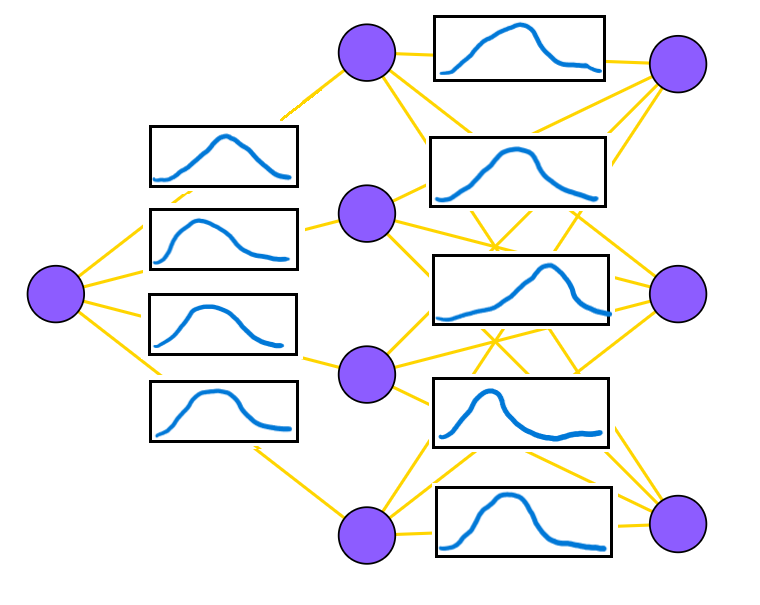
\includegraphics[width=.35\textwidth]{Figures/BNN_weightstoc.png}
    \caption{\footnotesize{A two-layer Bayesian Neural Network with parameters as distributions rather than strict point estimates.}}
  \label{BayesNet}
  \vspace{-10pt}
\end{wrapfigure}

 In the ``traditional'' neural network framework, to train a neural network to minimize its error based on a single point estimate for each $w_i$, waged against a cost function, is to maximize the likelihood of the training data (i.e. finding weights $w_i$ that maximize $P(D_{train}|W)$ \cite{bishop1995} \cite{bishop1997bayesian}.  The drawback to an ANN is that the distribution of network parameters $\theta = (W,b)$ across the network is unknown. \cite{mullachery2018bayesian}  Without supplemental engineering, measurements of the model's uncertainty cannot be quantified (as described earlier).
 
 In Bayes, there are no point estimates. Instead, by use of Bayes’ Rule, an interval of potential weights based on probabilities $p(w|D)$ is computed.  As such, the network can express uncertainty in its weights through this posterior distribution.  What's more is by the rudimentary feature of marginalization, uncertainty can be quantified for the predicted outputs $p(y|D)$ (for either $y$ as a regression prediction or classification label); even the very architecture of the model $p(A|D)$ can be expressed as a distribution. \cite{bishop1995}
 

\section{Architecture}

A researcher unsatisfied with a single point estimate for network outputs may consider simulating multiple networks, introducing a stochastic effect to parameter tuning so as to not generate the same results. Stochastic neural networks, which use either stochastic activations or stochastic weights, simulate multiple possible models $\theta$ with associated probability distribution $p(\theta)$.  Aggregating independent predictors can lead to better predictions than single point estimates. \cite{Jospin}.  In comparing the predictions of multiple samples of $\theta$, stochastic models better measure uncertainty.  Bayesian neural networks are a special case of stochastic neural networks in which the ensemble of possible models is obtained using Bayesian inference. \cite{mackay1992practical}

\subsection{Stochastic Modeling} B
JOSPIN, page 5

Stochastic neural networks are ANN's with a stochastic element introduced into the model.  A simple example is the regularization technique dropout \cite{goan2020bayesian} described earlier.  A neural network trained with dropout has a component randomness introduced by the selection of neurons removed from training.  If the dropout model was trained over and over again, it would contain slightly different parameter values reflective of this random noise.  There are other ways to introduce stochasticity into the model.  For example in regression, the network could assume residual normality by introducing Gaussian noise in its data generation \cite{Jospin}.  That is, for parameterizing weights $w$:
\begin{gather*}
\theta \sim N(\mu,\sigma^2) \\
w \sim p(w|D_{train},\theta)
\end{gather*}

This is the essence of how a BNN is a special case of a stochastic model.  The difference lies in that the stochastic element $\theta$ lies in the prior $p(\theta)$.

\subsection{Selection of Priors}

\textit{(Refer back to "From Prior to Posterior" and reiterate how to select priors for BNN's, specifically)}

There is no one-size-fits-all for machine learning models, and deep learning models only inflate this fact due to their enormous complexity \cite{Goodfellow-et-al-2016}.  Therefore, it can be interpreted \cite{Jospin} that prior assumptions are in place for all machine learning models, be it the optimization algorithm, regularizer, architecture, etc. These are implicit for non-Bayesian networks.  However, with Bayes, the prior assumptions are made explicit.  Yet, by the same logic, it is not always intuitive how to select priors.  A beginner's start for a regression task is to select a normal prior $p(\theta) \sim N(\mu,\sigma^2)$.  This is analogous to the point-estimate weight decay regularization described in earlier sections, but will be further discussed later in this section. \textbf{DO THIS and ensure the same notation}  Despite this, there is no theoretical argument that makes a normal prior better than any other \cite{silvestro2020prior}; it simply has nice mathematical properties.


\subsection{Development}

\textit{(Add more here.  Introduce the prior selected from the last subsection and incorporate more steps to reaching the posterior)}

Recall that $\theta$ represents the model weights and biases $(W,b)$.  $D$ is the training data from which the model learns, its inputs and outputs denoted with sibscripts $_x$ and $_y$.  Applying Bayes' Theorem, to determine the posterior distribution of $\theta$ requires selection of a prior and determination of the likelihood of the data:

$$
p(\theta|D) = \frac{p(D_{y}|D_{x},\theta)p(\theta)}{\int_\theta p(D_{y}|D_{x},\theta')p(\theta')d\theta'}
$$

The normalizing constant in the denominator is what has been seen before: the difficult (profoundly intractable for any informative BNN's) integral that requires estimation by Markov Chain Monte Carlo or variational inference.

\textit{(lead into the next subsection)}

\subsection{Inference}

\textit{(Add more into this section.  Check a reference, first, to see what I can add...)}

Marginalization takes reign when determining the distribution of network predictions.  This means integrating out $\theta$ from the final model.  Given the posterior distribution of network parameters $p(\theta|D)$, the distribution of network predictions $p(y|x,D)$ is calculated as:
$$
p(y|x,D) = \int_\theta p(y|x,\theta')p(\theta'|D)d\theta'
$$

Usually in practice, a collection of samples $\Theta$ is taken from $p(\theta|D)$ and $Y$ from $p(y|x,D)$ \cite{Jospin}. By this point the distributions have been approximated by MCMC. These samples are aggregated to measure uncertainty and generate an estimate $\hat{y}$.

%If $y = \Phi_{\theta} (x)+ \epsilon$ represents the 


\section{Performance Metrics}

\textit{(something here)}

\subsection{Description of Uncertainty}

A quick recap is in order for uncertainty definitions: \textit{Aleatoric} uncertainty is the level of uncertainty due to the noise or random variation of the data (i.e. error).  \textit{Epistemic} uncertainty is the measure of uncertainty a model has (i.e. variance).

BNN's allow for distinguishability between these types of uncertainty \cite{Jospin}.  $p(\theta|D)$ measures the epistemic uncertainty in the model.  With few data points, the model will express a high level variation in its choice of parameters rather than blintly returning a seemingly confident answer.  With more data points, this uncertainty reduces.

Aleatoric uncertainty is measured by $p(y|x,\theta)$, which is the conditional probability of the predicted output given the input predictors and model parameters.  This conditional probability is not isolated to Bayesian models; however, use of Bayes provides a means of inverting conditional probabilities when necessary \cite{Jospin}.


Let $y = \Phi_{\theta} (x) + \epsilon$ represent the value of $y$ from the approximated distribution of parameter estimates (with error $\epsilon$) given input $x$.

For regression tasks, usually models are averaged to summarize BNN predictions: 
$$
\hat{y} = \frac{1}{|\Theta|} \sum_{\theta_i} \Phi_{\theta_i}(x)
$$

Uncertainty is computed by the \textit{covariance matrix}:
$$
\Sigma_{y|x,D} = \frac{1}{|\Theta|-1} \sum_{\theta_i} (\Phi_{\theta_i}(x) - \hat{y}) (\Phi_{\theta_i}(x) - \hat{y})^\intercal
$$

For classification tasks, the estimator is the most likely class, that is $\hat{p} = max(p_i)$.  Uncertainty is measured by the relative probability of each class, summarized by the average.
$$
\hat{p} = \frac{1}{|\Theta|} \sum_{\theta_i} \Phi_{\theta_i}(x)
$$

\subsection{Regularization}

\textit{(Inflate this section and give more evidence as to HOW BNN's prevent overfitting)}

ANN's built from a non-Bayesian approach aim to minimize a loss function.  As mentioned earlier, this is that maximizes the likelihood of the data.  Mathematically:
$$
min(E_D(D|\theta)) = max(p(D_y|D_x,\theta)
$$
(For notational symmetry, $E_D(D|w,A)$ as was described in previous sections is now represented as $E_D(D|\theta)$)

Non-Bayesian networks introduce a regularizing term to prevent issues of overfitting.  In Bayes, the selection of a prior acts as the regularizing term \cite{Jospin},  That is:
$$
 max(p(D_y|D_x,\theta) = min(E_D(D|\theta) + E_{\Theta}(\theta)
$$
Where $E_{\theta}(\theta)$ is the new representation of $E_W(w|A)$ from earlier sections.

\section{Infinity and Beyond}

\subsection{Model Comparison}
As promised at the beginning of this chapter, Bayes can be applied to select an ideal capacity model \cite{bishop1997bayesian}.  Consider three networks of different capacities.  Better yet, take the three networks from the Tohoku Earthquae example, each with an additional hidden layer.  Now, suppose they are Bayesian networks represented as $B_1, B_2, B_3$ with the subscript representing the number of hidden layers (an analogous simulation may be in the works for future projects).
$$
p(B_i|D) = \frac{p(D|B_i)p(B_i)}{p(D)}
$$
Without justification to prefer one model over the other, the prior $p(B_i)$ would be the same.  Therefore, the complexity of the model is contingent only upon the data likelihood under each model $p(D|B_i)$.  Different models can be compared; the model with the highest likelihood of the data has better evidence for its predictions.

\begin{figure}[H]
    \centering
    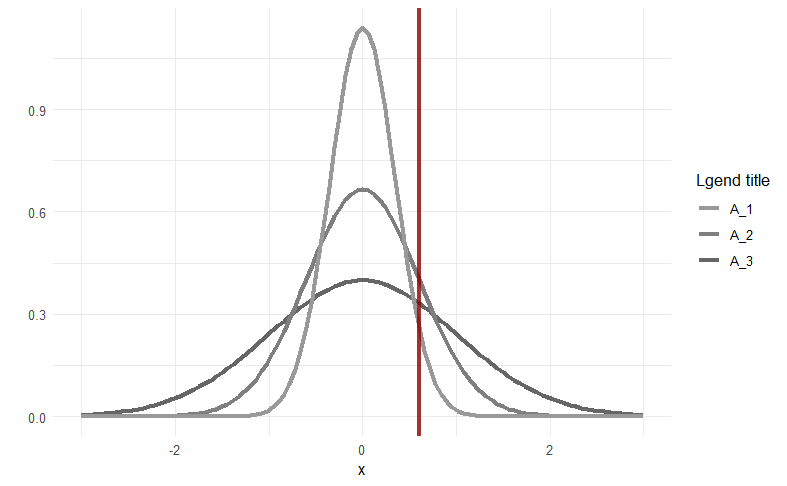
\includegraphics[width = .6\textwidth]{Figures/BNN_modelcheck.png}
    \caption{\footnotesize{ADD A DESCRIPTIVE CAPTION HERE}}
    \label{BNNmodelcheck}
\end{figure}

\subsection{Mixed Networks}
Just as a Convolutional Neural Network is simply any neural network which incorporates the convolution operation, so too can a Bayesian component of a neural network be limited to just one layer.

\subsection{Bayesian Teachers}
Jospin p. 14


\begin{comment}
\section{Fitting a BNN}

Final run at the Tohoku Earthquake example that fits an \textit{ACTUAL} BNN with plenty of performance metrics displayed.


Each Subsection will be the main steps as shown in my R code.
\end{comment}